\documentclass[a4paper,11pt]{article}
\usepackage{ctex}
\usepackage{enumerate}
\usepackage{times}
\usepackage{mathptmx}
\usepackage{amsmath}
\usepackage{amssymb}
\usepackage{tikz}
\usepackage{clrscode3e}
\usepackage[top=2cm, bottom=2cm, left=2cm, right=2cm]{geometry}

\allowdisplaybreaks[4]
\renewcommand{\labelenumi}{\textbf{\emph{\alph{enumi}}.}}
\begin{document}
  \title{����~2-11~��ҵ}
  \author{��������ۿԴ \and ѧ�ţ�161240004}
  \date{}
  \maketitle

  \section{[TC] Problem 12.1-2}
  In a binary search tree, every node is greater than or equal to all the elements in its left subtree, and is less than or equal to all the elements in its right subtree. However, in a min-heap, every node is less than or equal to its child(ren), both left and right, if exist. \par
  Min-heap property can not be used to print out the keys in sorted order in $O(n)$ time. If it can, then we sort the $n$ keys in $O(n)$ time, because building an $n$-node heap only takes a running time of $O(n)$, and this is contradictory to the $\Omega(n \log n)$ lower bound for comparison-based sorting algorithm.

  \section{[TC] Problem 12.1-5}
  Suppose, to the contrary, that there exists a comparison-based algorithm, that constructs an $n$-element binary search tree in $o(n \log n)$ time. We use this algorithm to build a binary search tree. The inorder traversal of the binary search tree gives the list of all the elements in the tree in sorted order, and it takes a running time of $O(n)$. That means, we can sort $n$ elements in $o(n \log n)$ running time, which is contradictory
  to the $\Omega(n \log n)$ lower bound for comparison-based sorting algorithm.

  \section{[TC] Problem 12.2-5}
  When a node in a binary search tree has two children, then its successor is the minimum element in its right subtree. In \proc{Tree-Minimum}, line 1, the \While loop condition ``$\attrib{x}{left} \neq \const{nil}$'' guarantees that when the loop terminates, the minimum element, $x$ must not have a left child. \par
  Likewise, the predecessor is the maximum element in its left subtree, and the \While loop condition in \proc{Tree-Maximum} guarantees that the maximum element must not have a right child.

  \section{[TC] Problem 12.2-8}
  The $k$ successive calls to \proc{Tree-Successor} output a consecutive subsequence of the inorder traversal of the tree. During this process, every node, say $x$, in the tree, is visited at most three times: entering the tree rooted in $x$ from its parent, then visiting its left subtree; leaving its left subtree, outputting $x$ itself, and then visiting its right subtree; leaving the right subtree, then returning to its parent. The $k$ elements visited and outputted takes a running time of $O(k)$. Now, we are going to consider the elements visited but not outputted. \par
  Assume, the lowest common ancestor of the outputted elements is $a$, then $a$ must be outputted according to the binary search tree property. In the left subtree of $a$, we claim that there do not exist two elements $b_1, b_2$ at the same level visited but not outputted. Otherwise, let $a'$ be their lowest common ancestor, and assume $b_1$ is in the left subtree of $a'$ and $b_2$ is in the right one. Since both $b_1$ and $b_2$ have been visited, the procedure must have left the left subtree of $a'$ and entered the right subtree of $a'$, and thus $a'$ must have been outputted. Now, we have proved that both $a$ and $a'$ have been outputted, but $b_2$, between $a$ and $a'$, is not outputted, which leads to a contradiction.
  So, there are at most $h$ elements visited but not outputted in the left subtree of $a$, and they take a running time of $O(h)$. Likewise the elements visited but not outputted in the right subtree of $a$ take a running time of $O(h)$. \par
  Therefore, the total running time is $O(k+h)$.

    \vspace{0.3cm}
  \scriptsize
  \begin{centering}
  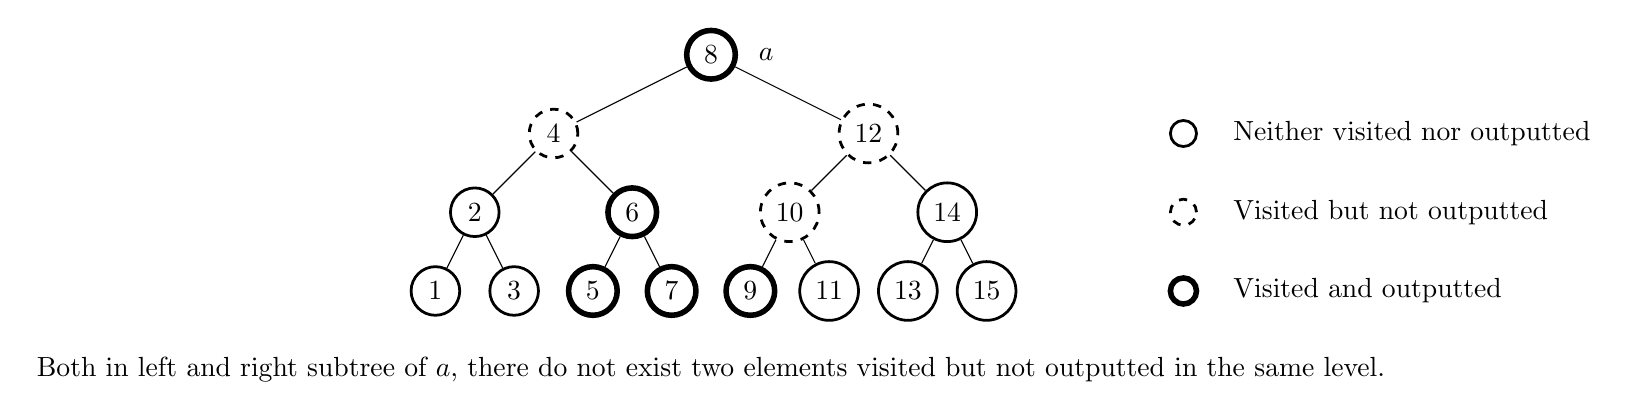
\begin{tikzpicture}[line width = 1pt,
                    solid/.style = {circle, draw, fill = black, minimum size = 0.3cm},
                    empty/.style = {circle, draw, fill = white, minimum size = 0.3cm}]
  \node at (6.7,0) {$a$};
  \node [empty, line width = 2pt] (T01) at (6,0) {8};
  \node [empty, dashed] (T11) at (4,-1) {4};
  \node [empty, dashed] (T12) at (8,-1) {12};
  \node [empty] (T21) at (3,-2) {2};
  \node [empty, line width = 2pt] (T22) at (5,-2) {6};
  \node [empty, dashed] (T23) at (7,-2) {10};
  \node [empty] (T24) at (9,-2) {14};
  \node [empty] (T31) at (2.5,-3) {1};
  \node [empty] (T32) at (3.5,-3) {3};
  \node [empty, line width = 2pt] (T33) at (4.5,-3) {5};
  \node [empty, line width = 2pt] (T34) at (5.5,-3) {7};
  \node [empty, line width = 2pt] (T35) at (6.5,-3) {9};
  \node [empty] (T36) at (7.5,-3) {11};
  \node [empty] (T37) at (8.5,-3) {13};
  \node [empty] (T38) at (9.5,-3) {15};

  \node [empty] at (12, -1){};
  \node [right] at (12.5, -1) {Neither visited nor outputted};
  \node [empty, dashed] at (12, -2){};
  \node [right] at (12.5, -2) {Visited but not outputted};
  \node [empty, line width = 2pt] at (12, -3){};
  \node [right] at (12.5, -3) {Visited and outputted};

  \node at (6, -4) {Both in left and right subtree of $a$, there do not exist two elements visited but not outputted in the same level.};
  \draw [thin] (T01) -- (T11);
  \draw [thin] (T01) -- (T12);
  \draw [thin] (T11) -- (T21);
  \draw [thin] (T11) -- (T22);
  \draw [thin] (T12) -- (T23);
  \draw [thin] (T12) -- (T24);
  \draw [thin] (T21) -- (T31);
  \draw [thin] (T21) -- (T32);
  \draw [thin] (T22) -- (T33);
  \draw [thin] (T22) -- (T34);
  \draw [thin] (T23) -- (T35);
  \draw [thin] (T23) -- (T36);
  \draw [thin] (T24) -- (T37);
  \draw [thin] (T24) -- (T38);
  \end{tikzpicture} \par
  \end{centering}
  \normalsize

  \section{[TC] Problem 12.2-9}
  If $x$ is the left child of $y$, since $x$ is a leaf, $x$ is the rightmost node in $x$'s left subtree, so $\attrib{x}{key}$ is the largest key in $T$ smaller than $\attrib{y}{key}$, i.e. $\attrib{y}{key}$ is the smallest key in $T$ larger than $\attrib{x}{key}$. \par
  If $x$ is the right child of $y$, $x$ is the leftmost node in $x$'s right subtree because $x$ is a leaf, so $\attrib{x}{key}$ is the smallest key in $T$ larger than $\attrib{y}{key}$, i.e. $\attrib{y}{key}$ is the largest key in $T$ smaller than $\attrib{x}{key}$.

  \section{[TC] Problem 12.3-5}
  \begin{codebox}
  \Procname{$\proc{Parent}(T, x)$}
  \li $y \gets x$
  \li \While $\attrib{y}{right} \neq \const{nil}$
  \li \Do $y \gets \attrib{y}{right}$
      \End
  \li $y \gets \attrib{y}{succ}$
  \li \If $y \neq \const{nil}$ and $\attrib{y}{left} \isequal x$
      \Comment $x$ is the left child of its parent
  \li \Do \Return $y$
  \li \Else \Comment $x$ is the right child of its parent
  \li    \If $y \isequal \const{nil}$
  \li    \Do $y \gets \attrib{T}{root}$
  \li    \Else
  \li        $y \gets \attrib{y}{left}$
         \End
  \li    \While $\attrib{y}{right} \neq x$
  \li    \Do $y \gets \attrib{y}{right}$
         \End
  \li    \Return $y$
      \End
  \end{codebox}
  \begin{codebox}
  \Procname{$\proc{Tree-Search}(x, k)$}
  \li \If $x \isequal \const{nil}$ or $k \isequal \attrib{x}{key}$
  \li \Do \Return $x$
      \End
  \li \If $k < \attrib{x}{key}$
  \li \Do \Return $\proc{Tree-Search}(\attrib{x}{left}, k)$
  \li \Else \Return $\proc{Tree-Search}(\attrib{x}{right}, k)$
  \end{codebox}
  TODO:
%  \begin{codebox}
%  \Procname{$\proc{Tree-Insert}(T, z)$}
%  \li $y \gets \const{nil}$
%  \li $x \gets \attrib{T}{root}$
%  \li \While $x \neq \const{nil}$
%  \li \Do $y \gets x$
%  \li     \If $\attrib{z}{key} < \attrib{x}{key}$
%  \li     \Do $x \gets \attrib{x}{left}$
%  \li     \Else $x \gets \attrib{x}{right}$
%          \End
%      \End
%  \li \If $y \isequal \const{nil}$
%  \li \Do $\attrib{T}{root} \gets z$
%  \li     $\attrib{z}{succ} \gets \const{nil}$
%  \li \ElseIf $\attrib{z}{key} < \attrib{y}{key}$
%  \li \Do $\attrib{z}{succ} \gets y$
%  \li     $x \gets \proc{Tree-Predecessor}(y)$
%  \li     \If $x \neq \const{nil}$
%  \li     \Do $\attrib{x}{succ} \gets z$
%          \End
%  \li \Else
%  \li     $\attrib{z}{succ} \gets \attrib{y}{succ}$
%  \li     $\attrib{y}{succ} \gets z$
%  \end{codebox}

  \section{[TC] Problem 12-1}
  \begin{enumerate}
    \item When all the keys are identical, the binary search tree is degenerate, i.e. it becomes a linked list, so inserting $n$ items with identical keys into an initially empty binary search tree takes a running time of $O(n^2)$.
    \item The binary search tree is balanced, because this strategy ensures that, for every node, its larger subtree contains at most one more node than the other, which means, the height of an $n$-element tree is $\lceil \lg (n+1) \rceil$. Inserting an element to a balanced tree of height $h$ runs in $O(h)$ time. Therefore, inserting $n$ identical elements takes a running time of
        $$ O\left(\sum_{i=1}^{n} \lceil \lg i \rceil \right) = O(n \lg n) $$
    \item We have only to insert the node to the head of the list, which takes $O(1)$ time, and inserting $n$ items takes $O(n)$ time in total.
    \item The worst case, is that, the tree is degenerate and becomes a linked list, and inserting $n$ items with identical keys takes a running time of $\Theta(n^2)$. \par
        To derive the expected running time, consider the empty children in the tree. Let $h_1, h_2, \cdots h_k$ denote the height of the empty children in an $n$-element tree. We claim that $k=n+1$ and $\sum_{i=1}^{n+1} (1/2)^{h_i} = 1$. This can be easily proved by mathematical induction: when the tree is empty, the only empty child is the root, whose height is 0; for any tree with $n$ elements, a leaf of of height $h$ just occupies a children of the tree without the leaf, but gives two new children of height $h+1$. \par
        The expected running time of inserting a node into an $n$-element binary search tree is $E(X) = \sum_{i=1}^{n+1} h_i(1/2)^{h_i}$. Substitution $H_i = (1/2)^{h_i}$ gives
        $$ E(X) = - \sum_{i=1}^{n+1} H_i \lg H_i \qquad \text{with} \quad \sum_{i=1}^{n+1} H_i = 1$$
        By Jensen's inequality, $E(X)$ is maximized when $H_1 = H_2 = \cdots = H_{n+1} = 1/(n+1)$, thus $E(X) \leq \lg (n+1) = O(\lg n)$. Therefore, the expected running time of inserting $n$ elements is $O(n \lg n)$.
        
        \vspace{0.3cm}
        \scriptsize
        \begin{centering}
        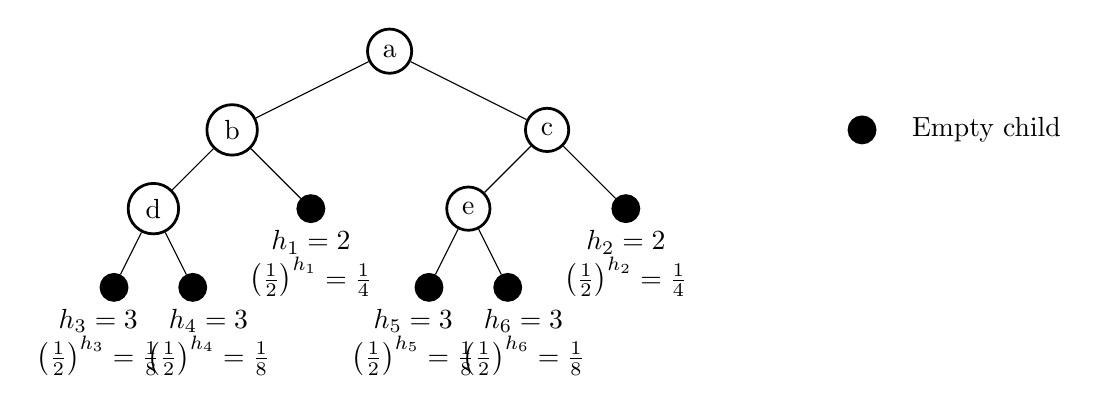
\begin{tikzpicture}[line width = 1pt,
                        solid/.style = {circle, draw, fill = black, minimum size = 0.3cm},
                        empty/.style = {circle, draw, fill = white, minimum size = 0.3cm}]
        \node [empty] (T01) at (6,0) {a};
        \node [empty] (T11) at (4,-1) {b};
        \node [empty] (T12) at (8,-1) {c};
        \node [empty] (T21) at (3,-2) {d};
        \node [solid] (T22) at (5,-2) {};    \node [align=center] at (5,-2.7) {$h_1=2$ \\ $\left(\frac{1}{2}\right)^{h_1} = \frac{1}{4}$};
        \node [empty] (T23) at (7,-2) {e};
        \node [solid] (T24) at (9,-2) {};    \node [align=center] at (9,-2.7) {$h_2=2$ \\ $\left(\frac{1}{2}\right)^{h_2} = \frac{1}{4}$};
        \node [solid] (T31) at (2.5,-3) {};  \node [align=center] at (2.3,-3.7) {$h_3=3$ \\ $\left(\frac{1}{2}\right)^{h_3} = \frac{1}{8}$};
        \node [solid] (T32) at (3.5,-3) {};  \node [align=center] at (3.7,-3.7) {$h_4=3$ \\ $\left(\frac{1}{2}\right)^{h_4} = \frac{1}{8}$};
        \node [solid] (T33) at (6.5,-3) {};  \node [align=center] at (6.3,-3.7) {$h_5=3$ \\ $\left(\frac{1}{2}\right)^{h_5} = \frac{1}{8}$};
        \node [solid] (T34) at (7.5,-3) {};  \node [align=center] at (7.7,-3.7) {$h_6=3$ \\ $\left(\frac{1}{2}\right)^{h_6} = \frac{1}{8}$};

        \node [solid] at (12, -1){};
        \node [right] at (12.5, -1) {Empty child};

        \draw [thin] (T01) -- (T11);
        \draw [thin] (T01) -- (T12);
        \draw [thin] (T11) -- (T21);
        \draw [thin] (T11) -- (T22);
        \draw [thin] (T12) -- (T23);
        \draw [thin] (T12) -- (T24);
        \draw [thin] (T21) -- (T31);
        \draw [thin] (T21) -- (T32);
        \draw [thin] (T23) -- (T33);
        \draw [thin] (T23) -- (T34);
        \end{tikzpicture} \par
        \end{centering}
        \normalsize
  \end{enumerate}
\end{document}
